\section{Theory}

	Cadmium has the electron structure, $(Kr)4d^{10}5s^2$, i.e. the outer shell taking part in optical transitions is composed of the two $5s^2$ electrons representing a completed electron shell. The transition used to demonstrate the normal Zeeman effect is $3^1 D_2 \rightarrow 2^1 P_1$ with $643.85nm$ and the transition used to demonstrate anomalous Zeeman effect is $2^3S_1 \rightarrow 2^3P_2$ with $508.58nm$. This has been shown in the \hyperref[fig:splitting]{Figure 1}.

	The anomalous Zeeman effect is the more general case where the electron spins do not cancel each other and the energy of an atomic state in a magnetic field depends on both the magnetic moments of electron orbit and electron spin. The spectrum after being filtered out is studied using a Fabry-Perot interferometer. With the magnetic field turned on in the absence of the analyser three lines can be seen simultaneously in the normal Zeeman effect in transversal observation. In the case of the anomalous Zeeman effect, three groups of three lines appear. Inserting the analyser in the normal Zeeman effect two $\sigma$ lines can be observed if the analyser is in the vertical position, while only the $\pi$ line appears if the analyser is turned into its horizontal position (transversal Zeeman effect). In the anomalous Zeeman effect, there are two groups of three $\sigma$ lines in vertical polarization and one group of three $\pi$ lines in horizontal polarization. Turning the magnetic system by $90^\circ$ the light coming from the spectral lamp parallel to the direction of the field (longitudinal) can also be studied through the holes in the pole pieces. It can be shown that this light is circularly polarized light (longitudinal Zeeman effect). A $\lambda/4$ plate is generally used to convert linear into elliptically polarized light. In this experiment, the $\lambda/4$ plate is used in the opposite way. With the $\lambda/4$ plate inserted before the analyser, the light of the longitudinal Zeeman effect is investigated. If the optical axis of the $\lambda/4$ plate coincides with the vertical, it is observed that some rings disappear if the analyser $45^\circ$ is at an angle of with the vertical while other rings disappear for a position of $45^\circ$. That means that the light of the longitudinal Zeeman effect is polarized in a circular (opposed way). The $\pi$ lines are longitudinally not observable.

	\begin{figure}[H]
		\centering
		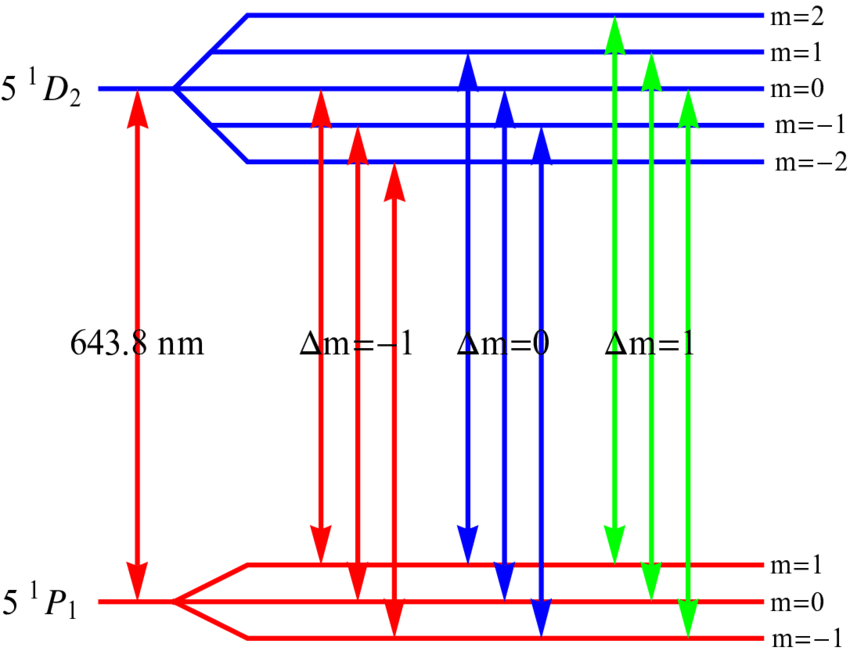
\includegraphics[width=0.8\columnwidth]{cd_splitting.png}
		\caption{Splitting of lines in cadmium}
		% \caption{\textbf{Splitting of lines in cadmium}}
		\label{fig:splitting}
	\end{figure}

	\subsection{Fabry-Perot interferometer}
		The Fabry-Perot interferometer uses the phenomenon of multiple beam interference that arises when light shines through a cavity bounded by two reflective parallel surfaces. Each time the light encounters one of the surfaces, a portion of it is transmitted out, and the remaining part is reflected back. The net effect is to break a single beam into multiple beams which interfere with each other. If the additional optical path length of the reflected beam (due to multiple reflections) is an integral multiple of the light's wavelength, then the reflected beams will interfere constructively. More is the number of reflection inside the cavity, sharper is the interference maximum. 


		\begin{figure}[H]
			\centering
			\fbox{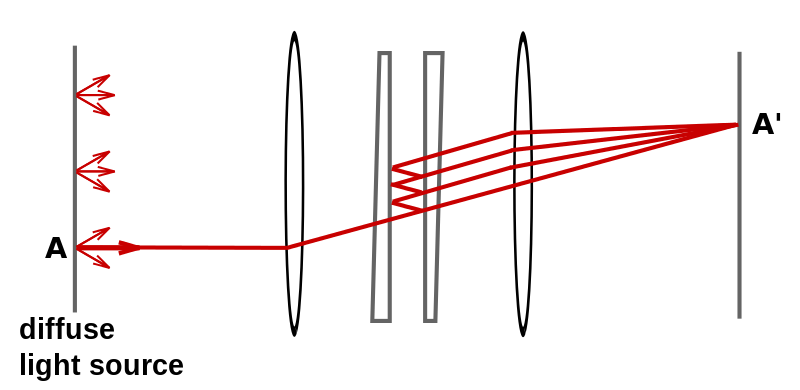
\includegraphics[width=\columnwidth]{interferometer.png}}
			%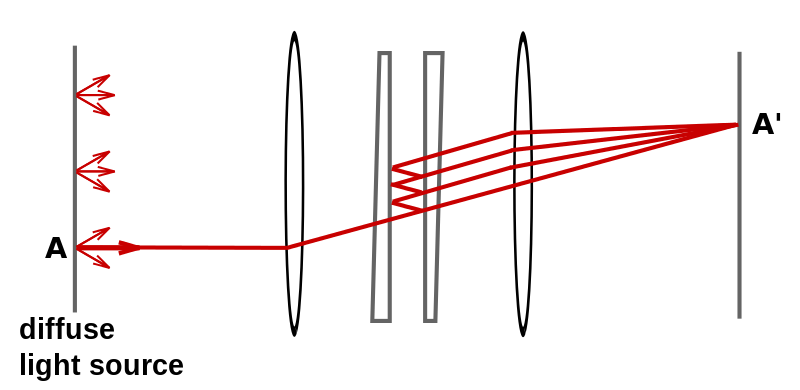
\includegraphics[height=5cm]{interferometer.png}
			\caption{Interferometer working}
			% \caption{\textbf{Interferometer working}}
			\label{fig:interferometer}
		\end{figure}
		It makes use of multiple reflections which follow the interference condition for thin films. The net phase change is zero for two adjacent rays, so the relation to find a maxima is:

		\begin{equation}
			2d\cos\theta = n\lambda
		\end{equation}

		\begin{figure}[H]
			\centering
			\fbox{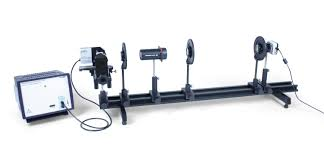
\includegraphics[width=\columnwidth]{setup.jpg}}
			%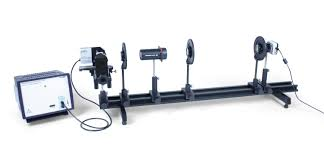
\includegraphics[height=5cm]{setup.jpg}
			\caption{Experimental setup}
			% \caption{\textbf{Experimental setup}}
			\label{fig:setup}
		\end{figure}